\documentclass[12pt,a4paper]{report}
%
% This LaTeX template has been created by Luca Grilli
% Based on the following https://en.wikibooks.org/wiki/LaTeX/Title_Creation
%
\usepackage[italian]{babel}
%\usepackage[T1]{fontenc} % Riga da commentare se si compila con PDFLaTeX
\usepackage{geometry}
\usepackage{graphicx}
\usepackage{hyperref}
\usepackage[utf8]{inputenc}
\usepackage{lipsum} % genera testo fittizio
\usepackage{subcaption}
\usepackage[nottoc,numbib]{tocbibind}
\usepackage{titlesec}

\titleformat{\chapter}[display]{\Huge\bfseries}{}{0pt}{\thechapter.\ }

\graphicspath{{figures/}}
%
%\addtolength{\topmargin}{-.875in} % reduce the default top margin
%\addtolength{\topmargin}{-2cm} % reduce the default top margin
%



%%%%%%%%%%%%%%%%%%%%%%%%%%%%%%%%%%
%                                %
%     Begin Docuemnt [start]     %
%                                %
%%%%%%%%%%%%%%%%%%%%%%%%%%%%%%%%%%
\begin{document}



%%%%%%%%%%%%%%%%%%%%%%%%%%%%%%
%     Title Page [start]     %
%%%%%%%%%%%%%%%%%%%%%%%%%%%%%%
% Declare new goemetry for the title page only.
\newgeometry{margin=1in}
\begin{titlepage}
	\centering
	
\includegraphics[width=0.30\textwidth]{logo-unipg}\par\vspace{1cm}
	\large{Presentazione Progetto di}\par
	\large{\textbf{Programmazione di Interfacce Grafiche e Dispositivi Mobili}}\par
	\small{Corso di Laurea in Ingegneria Informatica ed Elettronica -- A.A. 2019-2020}\par
	\textsc{\small{Dipartimento di Ingegneria}}\par

	%\vfill
	\vspace{0.5cm}
	docente\par
	Prof.~Luca \textsc{Grilli}

	\vspace{1cm}
	\vspace{1cm}
	\textbf{\huge{JPacman}}\par
	\vspace{0.2cm}
	applicazione desktop \textsc{JFC/Swing}\par
	\vspace{0.5cm}
	
\includegraphics[width=0.30\textwidth]{jpacman-icon}\par\vspace{1cm}
	\vspace{1cm}

	\large{studenti}\par
	\vspace{0.2cm}
	\begin{tabular}{ l l l l }
	\large{316649} & \large{\textbf{Francesca}} & \large{\textbf{Nocentini}} & \large{francesca.nocentini@studenti.unipg.it}\\
	\large{312294} & \large{\textbf{Paolo}} & \large{\textbf{Speziali}} & \large{paolo.speziali@studenti.unipg.it}\\
	\end{tabular}

	%\begin{tabular}{ l l l l }
	%112233 & Francesca & Nocentini & francesca.nocentini@studenti.unipg.it\\
	%114455 & Paolo & Speziali & paolo.speziali@studenti.unipg.it\\
	%\end{tabular}

	\vfill
	% Bottom of the page
	%{\large \today\par}
	\raggedright
	\small{Data ultimo aggiornamento: \today}
\end{titlepage}
% Ends the declared geometry for the titlepage
\restoregeometry
%%%%%%%%%%%%%%%%%%%%%%%%%%%%
%     Title Page [end]     %
%%%%%%%%%%%%%%%%%%%%%%%%%%%%

%%%%%%%%%%%%%%%%%%%%%%%%%%
%     Indice [start]     %
%%%%%%%%%%%%%%%%%%%%%%%%%%
\tableofcontents
%%%%%%%%%%%%%%%%%%%%%%%%
%     Indice [end]     %
%%%%%%%%%%%%%%%%%%%%%%%%

%%%%%%%%%%%%%%%%%%%%%%%%%%%%%%%%%%%%%%%%%%%%
%     Descrizione del Problema [start]     %
%%%%%%%%%%%%%%%%%%%%%%%%%%%%%%%%%%%%%%%%%%%%
\chapter{Descrizione del Problema}\label{ch:despro}
L'obiettivo di questo lavoro è lo sviluppo di un'applicazione desktop, denominata \emph{JPacman}, che realizza una versione graficamente e strutturalmente semplificata dell'omonimo videogioco di casa Namco~\cite{wiki:it:pacman,wiki:it:namco}.

L'applicazione sarà implementata utilizzando la tecnologia JFC/Swing in modo da favorire un'ampia portabilità su diversi sistemi operativi (piattaforme), riducendo al minimo eventuali modifiche al codice sorgente. Il codice prodotto sarà testato e ottimizzato per la piattaforma Windows 10.

%----------------------------------------------
% Sezione: Il Videogioco Arcade Pac-Man [start]
%----------------------------------------------
\section{Il Videogioco Arcade Pac-Man}\label{se:gal}
Il giocatore deve guidare una creatura sferica di colore giallo, chiamata Pac-Man, facendole mangiare tutti i numerosi puntini disseminati ordinatamente all'interno del labirinto e, nel far questo, deve evitare di farsi toccare da quattro fantasmi, che alternano la loro modalità Inseguimento (Chase) con quella di Spargimento (Scatter)~\cite{pacmanai}., pena la perdita immediata di una delle vite a disposizione. Per facilitare il compito al giocatore sono presenti, presso gli angoli dello schermo di gioco, quattro pillole speciali (\emph{PowerPills}) che rovesciano la situazione rendendo vulnerabili i fantasmi (modalità Frightened), che diventano blu e, per 10 secondi esatti, invertono la loro marcia; per guadagnare punti, è possibile in questa fase andare a caccia degli stessi fantasmi, per mangiarli.
Una volta fagocitati, però, questi tornano alla base (il rettangolo al centro dello schermo) sotto forma di un paio di occhi (modalità Eaten), per rigenerarsi e attaccare di nuovo Pac-Man. Completato un labirinto attraverso la fagocitazione di tutti i puntini, Pac-Man passa a quello successivo, identico nella struttura. I fantasmini hanno ognuno un comportamento differente nella modalità Chase:
\begin{itemize}
\item \textbf{Blinky} (Rosso): Il suo bersaglio è la posizione di Pac-Man;
\item \textbf{Pinky} (Rosa): Il suo bersaglio è quattro caselle di fronte a Pac-Man verso la direzione cui egli si sta muovendo;
\item \textbf{Inky} (Celeste): Il suo bersaglio è, preso come riferimento la lunghezza della linea che congiunge \textbf{Blinky} con la seconda casella di fronte a Pac-Man, l'estremità della linea lunga il doppio;
\item \textbf{Clyde} (Arancione): Il suo bersaglio è la posizione di Pac-Man finchè non si avvicina di 8 caselle, quando ciò avviene il suo bersaglio diventa quello della sua modalità Scatter;
\end{itemize}
Nella modalità Scatter i bersagli dei fantasmini sono quattro punti (uno per fantasma) posti ai lati del labirinto.

\begin{figure}[hb!]
\begin{subfigure}{.32\textwidth}
  \centering
  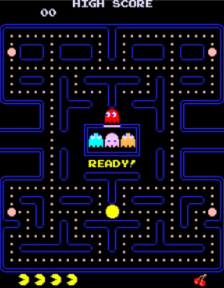
\includegraphics[width=.95\linewidth]{snapshot1}
  %\caption{1a}
  \caption{}
  \label{fig:snap1}
\end{subfigure}%
\begin{subfigure}{.32\textwidth}
  \centering
  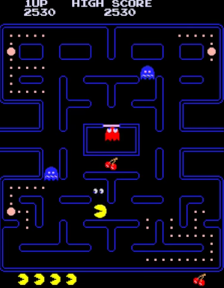
\includegraphics[width=.95\linewidth]{snapshot2}
  %\caption{1a}
  \caption{}
  \label{fig:snap2}
\end{subfigure}%
\begin{subfigure}{.32\textwidth}
  \centering
  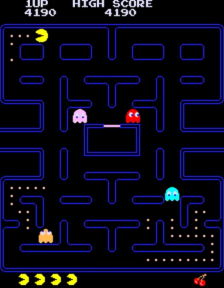
\includegraphics[width=.95\linewidth]{snapshot3}
  %\caption{1b}
  \caption{}
  \label{fig:snap3}
\end{subfigure}
\caption{Tre schermate del videogioco Pac-Man originale. La schermata (a) mostra l'inizio di una nuova partita. La schermata (b) mostra due fantasmi che scappano spaventati da Pac-Man dopo che questo ha mangiato una PowerPill, un fantasma rinato che torna all'inseguimento e un fantasma appena mangiato da Pac-Man che torna alla base. La schermata (c) mostra una partita quasi giunta alla conclusione.}
\label{fig:fig}
\end{figure}


%----------------------------------------------
% Sezione: Il Videogioco Arcade Pac-Man [end]
%----------------------------------------------



%----------------------------------------
% Sezione: L'applicazione JPacman [start]
%----------------------------------------
\section{L'applicazione JPacman}\label{se:appjgal}
L'applicazione JPacman replica in maniera fedele il gameplay del gioco originale.
I quattro fantasmi adottanno il comportamento classico Chase, Scatter, Frightened ed Eaten che era originariamente previsto, senza gli errori di movimento presenti nel cabinato originale (riferimento erroneamente spostato di alcune caselle se Pac-Man è rivolto verso l'alto). L'unica differenza dal gioco originale è la mancanza delle animazioni ``sketch" intermedie tra livelli.
%----------------------------------------
% Sezione: L'applicazione JPacman [end]
%----------------------------------------
%%%%%%%%%%%%%%%%%%%%%%%%%%%%%%%%%%%%%%%%%%
%     Descrizione del Problema [end]     %
%%%%%%%%%%%%%%%%%%%%%%%%%%%%%%%%%%%%%%%%%%



%%%%%%%%%%%%%%%%%%%%%%%%%%%%%%%%%%%%%%%%%%%
%     Specifica dei Requisiti [start]     %
%%%%%%%%%%%%%%%%%%%%%%%%%%%%%%%%%%%%%%%%%%%
%{\let\clearpage\relax \chapter{Specifica dei Requisiti}\label{ch:spereq}}
\chapter{Specifica dei Requisiti}\label{ch:spereq}

L'applicazione JPacman che si intende realizzare dovrà soddisfare i seguenti requisiti.

\begin{enumerate}
  \item Ricreare un labirinto in cui il personaggio e i nemici possano muoversi.
  \item Creare i quattro differenti nemici con i comportamenti del gioco originale (Chase/Scatter/Frightened/Eaten).
  \item Popolare il labirinto con le caratteristiche pillole e permettere al personaggio di raccoglierle ed accumulare punteggio.
  \item Popolare il labirinto con le caratteristiche PowerPill che permettono il passaggio alla modalità Frightened.
  \item Implementare un sistema di registrazione del punteggio.
  \item Implementazione delle animazioni di movimento e morte sia di Pac-Man che dei fantasmi.
  \item Popolare il labirinto con la caratteristica frutta per accumulare punteggio.
  \item Presenza di un sottofondo musicale e di effetti sonori attivabili/disattivabili dal pannello di configurazione dell’applicazione.
  \item Possibilità di metter in pausa il gioco con la pressione di un pulsante.
  \item Applicare un graduale aumento della difficoltà a seconda del livello raggiunto (fino ad un certo livello in cui si stabilizzerà).
  \item Arricchire il gioco con un movimento fluido dei personaggi all'interno del labirint.
  \item Inserimento di due scenari (labirinti) extra.
  \item Inserimento dei tunnel di teletrasporto nei labirinti \textit{(facoltativo)}.
  \item Aggiunta di un editor di livelli che permetta al giocatore di crearne di nuovi \textit{(facoltativo)}.
\end{enumerate}
%%%%%%%%%%%%%%%%%%%%%%%%%%%%%%%%%%%%%%%%%
%     Specifica dei Requisiti [end]     %
%%%%%%%%%%%%%%%%%%%%%%%%%%%%%%%%%%%%%%%%%

%%%%%%%%%%%%%%%%%%%%%%%%%%%%%%%%%%%%%%%%%%%%%
%     Bibliografia e Sitografia [start]     %
%                 NO BibTeX                 %
%%%%%%%%%%%%%%%%%%%%%%%%%%%%%%%%%%%%%%%%%%%%%
%\chapter{Bibliografia e Sitografia}\label{ch:bibsit}
%
%\begin{thebibliography}{9}
%\bibitem{lamport94}
%  Leslie Lamport,
%  \textit{\LaTeX: a document preparation system},
%  Addison Wesley, Massachusetts,
%  2nd edition,
%  1994.
%\end{thebibliography}
%
%%%%%%%%%%%%%%%%%%%%%%%%%%%%%%%%%%%%%%%%%%%
%     Bibliografia e Sitografia [end]     %
%                 NO BibTeX               %
%%%%%%%%%%%%%%%%%%%%%%%%%%%%%%%%%%%%%%%%%%%



%%%%%%%%%%%%%%%%%%%%%%%%%%%%%%%%%%%%%%%%%%%%%
%     Bibliografia e Sitografia [start]     %
%                with BibTeX                %
%%%%%%%%%%%%%%%%%%%%%%%%%%%%%%%%%%%%%%%%%%%%%
\bibliographystyle{plain}
\bibliography{bibliografia}
% inserire i riferimenti bibliografici nel file 'bibliografia.bib'
%%%%%%%%%%%%%%%%%%%%%%%%%%%%%%%%%%%%%%%%%%%
%     Bibliografia e Sitografia [end]     %
%                with BibTeX              %
%%%%%%%%%%%%%%%%%%%%%%%%%%%%%%%%%%%%%%%%%%%

\end{document}
%%%%%%%%%%%%%%%%%%%%%%%%%%%%%%%%
%                              %
%     Begin Docuemnt [end]     %
%                              %
%%%%%%%%%%%%%%%%%%%%%%%%%%%%%%%%